\documentclass[11pt, a4paper,titlepage]{report}
\usepackage{graphicx,epstopdf,titlesec,siunitx,chngcntr,fixltx2e,subcaption,appendix}
\usepackage{amsmath, bm, amssymb}
\usepackage{hyperref, fancyhdr, listings}
\usepackage{pdfpages, color}

\newcommand{\sectionbreak}{\clearpage}
\usepackage[authoryear]{natbib}
\usepackage{aas_macros, rotating, multirow, morefloats}
\usepackage[version=3]{mhchem}
\counterwithin{figure}{section}
\counterwithin{table}{section}
\newcommand\ion[2]{#1$\;${\scshape{#2}}}%
\newcommand{\Msun}{M$_{\odot}$~}
\newcommand{\Lagr}{\mathcal{L}}
\begin{document}

\begin{titlepage}
    \begin{center}
        
        \huge
        \textbf{NEMCEE  \\ The NEMESIS-EMCEE Interface}
        
        \vspace{0.5cm}
        \Large
        A no-nonsense guide and idiot-proof manual \\
        \vspace{1.0cm}
        
        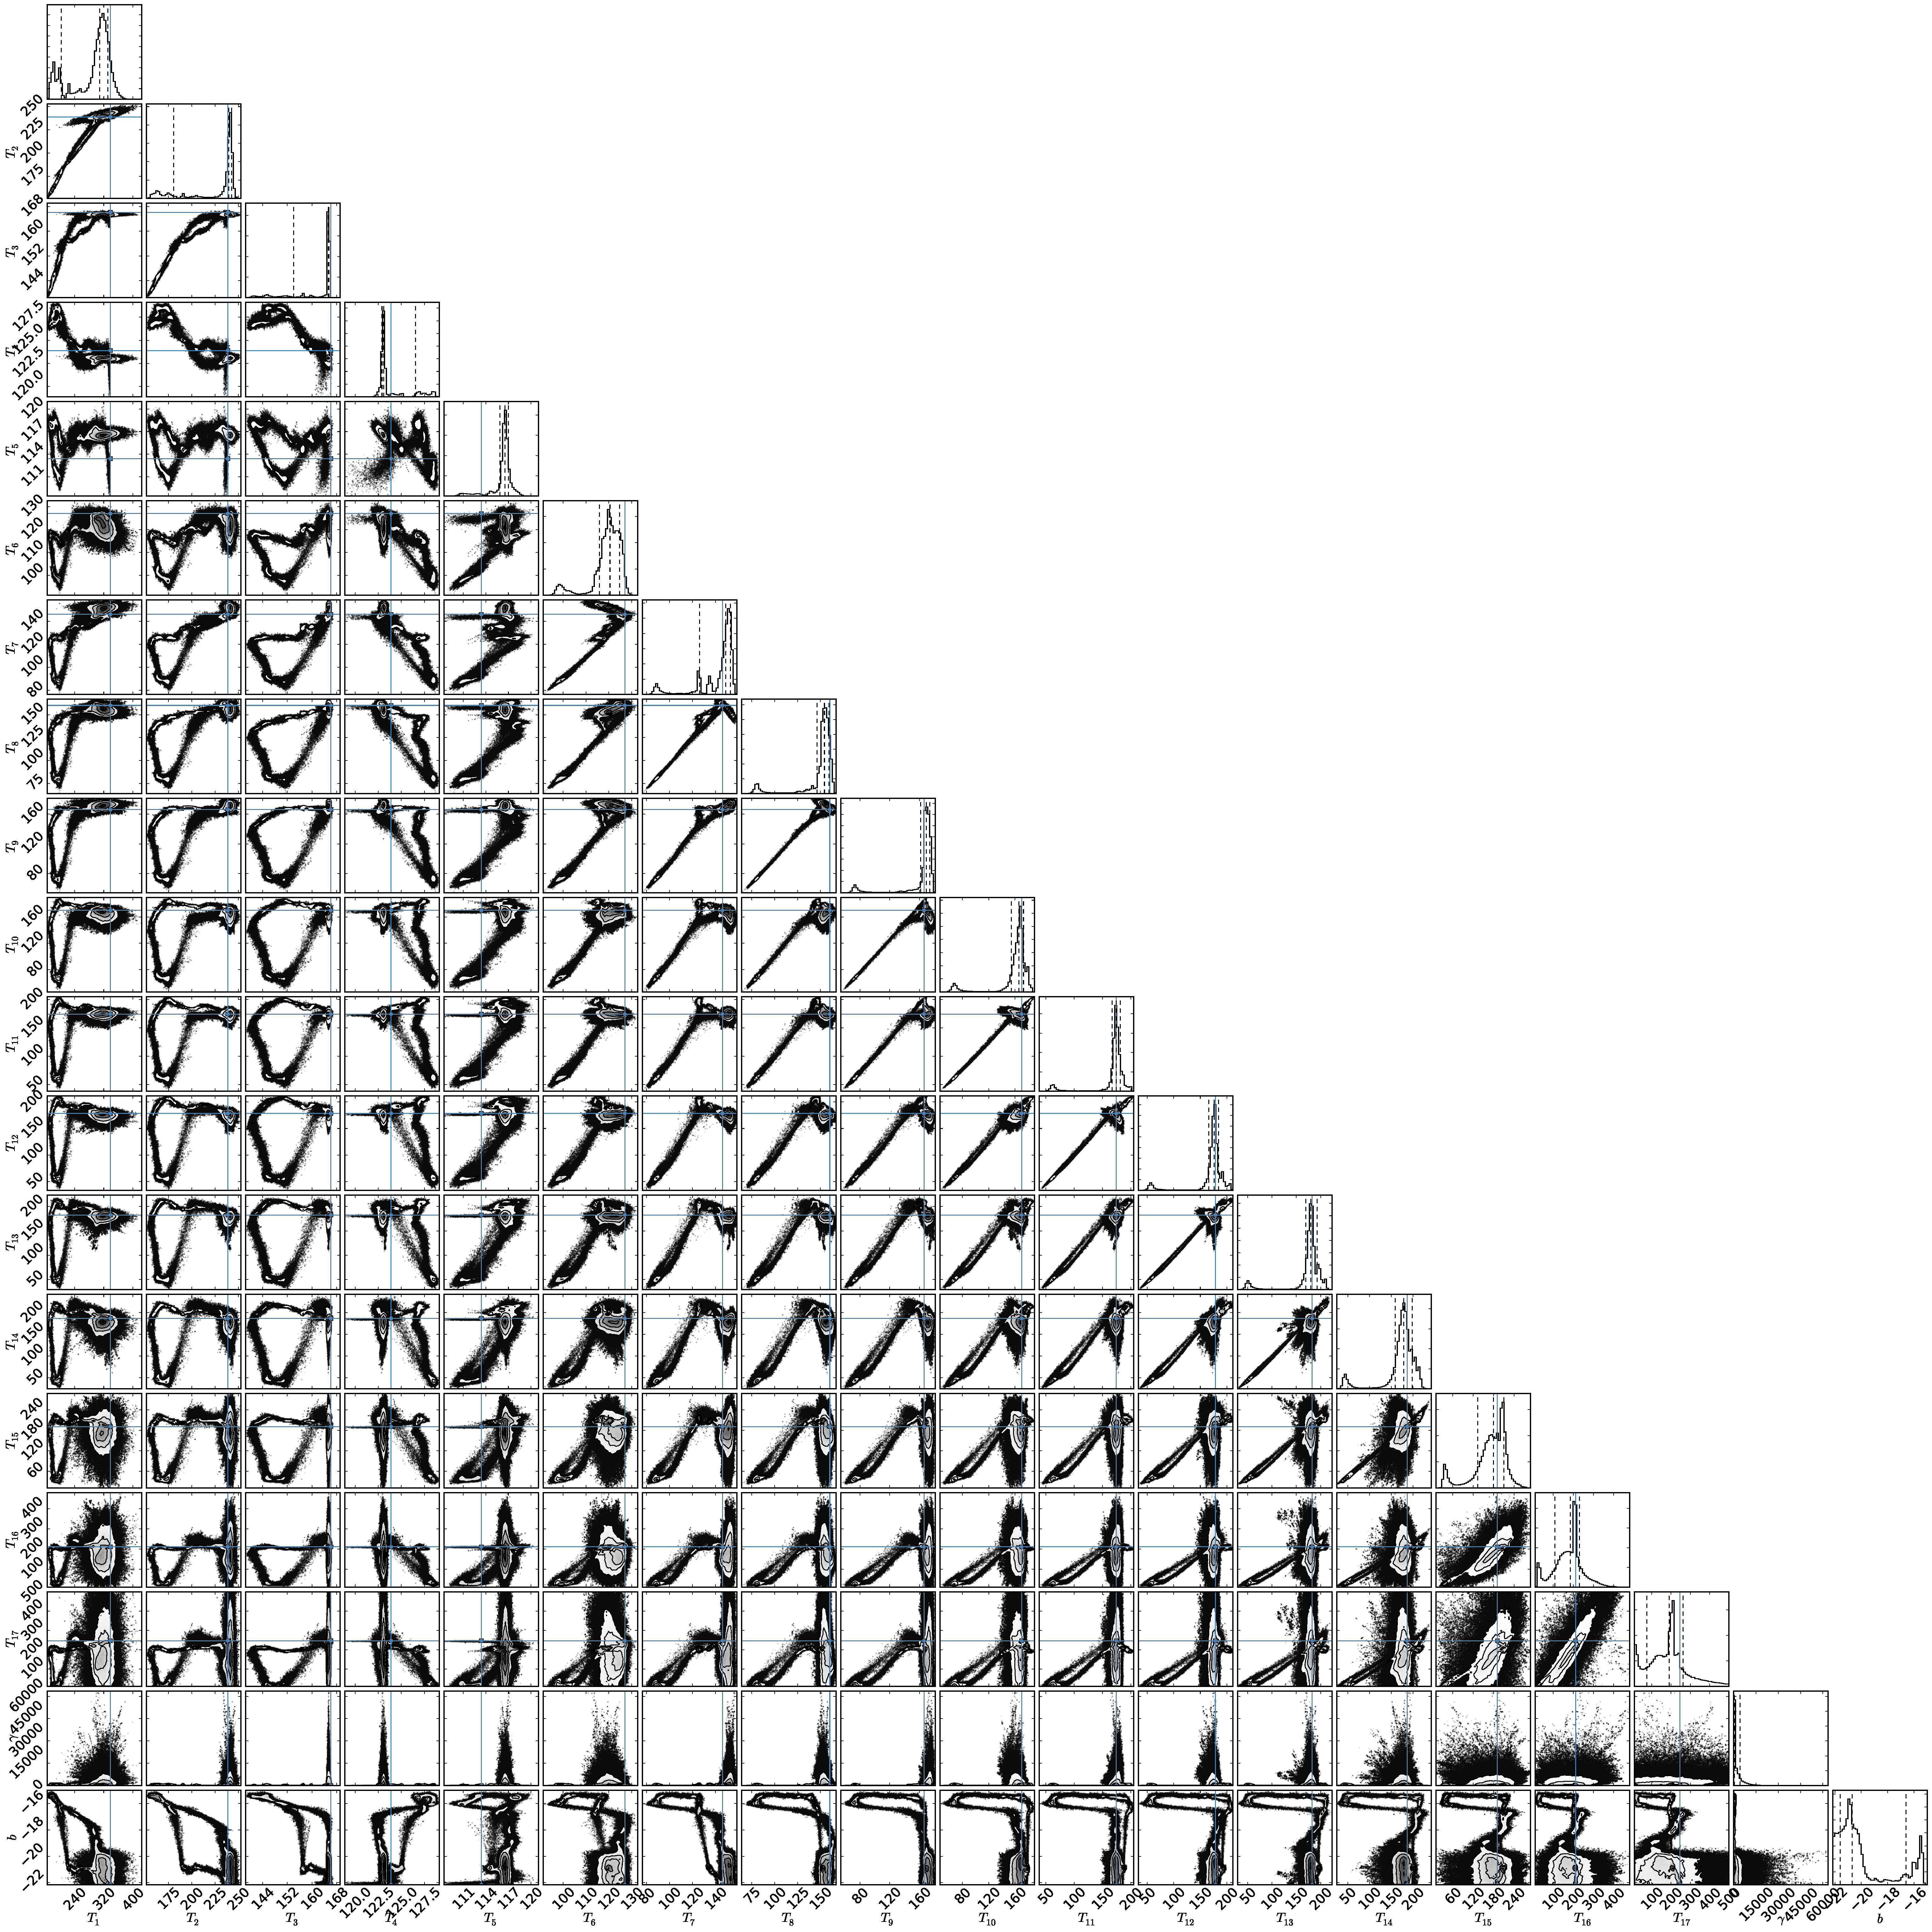
\includegraphics[width=1.0\textwidth]{100triangle}
        
        \vspace{1.5cm}        
	\LARGE
        \textbf{Ryan Garland} \\
          \Large
          ryan.garland@physics.ox.ac.uk
        
    \end{center}
\end{titlepage}

\tableofcontents

\newpage

\chapter{An Intro to EMCEE and MCMC}

This is taken from my first-year report and is only meant as a guide. If you truly want to get to grips with MCMC I'd recommend extensive googling and the Bayesian Data Analysis book by Gelman. For EMCEE, try Dan's website which contains a lot of info and links to the appropriate papers: http://dan.iel.fm/emcee/current/

\section{EMCEE}\label{section:emcee}

\subsection{Markov Chain Monte Carlo}

Bayesian inference is about the quantification and propagation of uncertainty, defined via a probability, in light of observations of the system. They arrive at a posterior probability distribution from an \textit{a priori} state vector. Markov Chain Monte Carlo (MCMC) techniques are methods for sampling from posterior probability distributions using Markov chains. 

The main reason why we are considering MCMC over optimal estimation is because of its ability to quantify all aspects of uncertainty via probability and propagate these errors robustly in the posterior probability distribution function. This is especially desirable for low resolution or wavelength-limited spectra, which is usually the case for Y dwarfs.

Consider the sequence of random \{$x_0 ,x_1 ,x_2 ,...$\} variables, sampled from the probability distribution $p(x_{t+1}|x_{t})$, then each next sample $x_{t+1}$ depends only on the current state $x_t$ and does not depend on the previous history \{$x_0 ,x_1 , ..., x_{t-1}$\}. Such a sequence is called a Markov chain. MCMC techniques aim to construct cleverly sampled chains which (after a burn-in period) draw samples which are progressively more likely realisations of the distribution of interest - the posterior probability distribution function (PDF). 

MCMC is a perfect match for planetary science, where the models are often expensive to calculate (because efficient sampling methods mean a lower amount of runs to realise the PDF), contain many free parameters, and have low signal-to-noise observations. MCMC has already been used to great effect by \citet{line15} to calculate the probability distribution functions of many relevant parameters to brown dwarf atmospheres, concluding that only low-resolution spectra are required to unambigously detect ammonia in T dwarfs. We note here that, in comparison to optimal estimation, MCMC can be orders of magnitude more computationally expensive. We are likely to therefore use both of these techniques alongside one another to determine atmospheric parameters. 

One of the key advantages of Bayesian data analysis is that it is possible to marginalise over nuisance parameters (e.g., spectral noise, instrumental errors).  A nuisance parameter is one that is required in order to model the process that generates the data, but is otherwise of little interest. Marginalisation is the process of integrating over all possible values of the parameter and hence propagating the effects of uncertainty about its value into the final result. 

Marginalisation is represented by the marginalised probability function $p(\Theta | D)$ of the set of model parameters $\Theta$ given the set of observations $D$:

\begin{equation}
p(\Theta | D)= \int p(\Theta, \alpha | D) \mathrm{d} \alpha
\end{equation}

where $\alpha$ is the set of nuisance parameters. Usually, the set $\alpha$ can be extremely large and therefore expensive to integrate. However an MCMC-generated sampling of values  $(\Theta_t,\alpha_t)$ (where $t$ is the timestep/iteration of the chain) of the model and nuisance parameters from the joint distribution $p(\Theta, \alpha | D)$ automatically provides a sampling of values $\Theta_t$ from the marginalised PDF $p(\Theta | D)$.

Another advantage of MCMC comes from the interest in the likelihood (or prior) function of the parameters, which may come from expensive calculations. Here, efficient MCMC sampling, where few function evaluations are required to create a statistically independent sample from the posterior PDF, is very valuable.  The methods presented here (Section~\ref{section:emcee}) are designed for efficiency.

\subsection{EMCEE} \label{section:emcee}

We use the Markov Chain Monte Carlo (MCMC) approach implemented with affine-invariant ensemble sampler EMCEE \citep{foreman-mackey13}, following \citet{line15}. Affine-invariant transformations preserve collinearity, so they transform parallel lines into parallel lines and preserve ratios of distances along parallel lines. Affine transformations allow the conversion of highly anisotropic probability distribution functions into isotropic distribution functions, which greatly reduces the difficulty of sampling the PDF. An algorithm that is affine invariant performs equally well under all linear transformations; it will therefore be insensitive to covariances among parameters. This is a significant advancement over the optimal estimation used previously in NEMESIS, as we are now able to make fewer \textit{a priori} assumptions, and the shape of the parameter uncertainties no longer need to be Gaussian. 

\subsubsection{Algorithm}

The EMCEE algorithm involves simultaneously evolving an ensemble of $K$ \textit{walkers} $S = \{X_k\}$ with positions X where the proposal distribution for one walker $k$ is based on the current positions of the $K - 1$ walkers in the \textit{complementary ensemble} $S_{[k]} = \{X_j , \forall j \neq k\}$. Here, position refers to a vector in the N-dimensional, real-valued parameter space.

To update the position of a walker at position $X_k$, a walker $X_j$ is drawn randomly from the remaining walkers $S_{[k]}$ and a new position $Y$ is proposed:

\begin{equation} \label{eqn:newpos}
X_{k(t)} \to Y = X_j + Z [X_{k(t)} - X_j]
\end{equation}

where Z is a random variable drawn from a distribution $g(Z = z)$:

\[g(z^{-1}) \propto \left\{
  \begin{array}{lr}
    \frac{1}{\sqrt{z}} & \mathrm{if} z \in \left[\frac{1}{a}, a \right]\\
    0 & \mathrm{otherwise}
  \end{array}
\right.
\]

and a is an adjustable scale parameter, normally set to 2. 

If $g$ satisfies

\begin{equation}
g(z^{-1}) = z g(z)
\end{equation}

the proposal of Equation~\ref{eqn:newpos} is symmetric in the sense that

\begin{equation} \label{eqn:detailedbalance}
p(X_{k}(t) \to Y) = p(Y \to X_{k}(t)).
\end{equation}

In this case, the chain will satisfy detailed balance (around any closed cycle of states, there is no net flow of probability, i.e. Equation~\ref{eqn:detailedbalance})
if the proposal is accepted with probability 

\begin{equation}
q = \mathrm{min} \left(1, Z^{N-1} \frac{p(Y)}{p(X_k (t))} \right)
\end{equation}

where $p(Y)$ is the probability of the proposed position $Y$, calculated from the likelihood function and the prior information described in sub-subsection~\ref{subsub:emceeint}, and $N$ is the dimension of the parameter space. This procedure is then repeated in series for each walker.

A huge benefit of using EMCEE, is that it may perform these iterations (with some modification to the algorithm) in parallel, and therefore the sampling may occur on multiple cores simultaneously, drastically reducing the amount of (real, not computational) time taken for each analysis. It is also configured for multicore-multinodal calculations using an MPI (message passing interface) setup, so that the calculations can be further spread between many computers and many cores at once.  

\subsubsection{NEMESIS Integration} \label{subsub:emceeint}

EMCEE requires a functional form for the log of the posterior probability to perform the sampling. The posterior probability is a combination of the likelihood and the prior described as follows. Starting from Bayes' theorem,

\begin{equation}
p(\bm{x} | \bm{y}) = \frac{\Lagr(\bm{y} | \bm{x}) p(\bm{x})}{E}
\end{equation}

where $\bm{x}$ is the parameter vector,  $\bm{y}$ is the data vector (i.e. the spectrum),  $p(\bm{x} | \bm{y})$ is the posterior probability distribution,  $\Lagr(\bm{y} | \bm{x})$ is the likelihood distribution which penalises poor/improbable fits to the data, $p(\bm{x})$ is the prior information which can restrict the parameter space, and E is the evidence, or marginal likelihood, which is a normalisation factor required for Bayesian model comparison, but not for parameter estimation, and is a complicated factor which requires sophisticated Monte Carlo methods to solve. We follow a similar method to \citet{line15}, describing the log-likelihood distribution with the function:

\begin{equation} \label{eqn:likelihood}
\mathrm{ln} \Lagr(\bm{y} | \bm{x}) = - \frac{1}{2} \displaystyle\sum_{i=1}^{n} \frac{(y_i - F_i(\bm{x}))^2}{s{_i}^2} - \frac{1}{2} \mathrm{ln}(2 \pi s{_i}^2)
\end{equation}


where the index $i$ denotes the $i$th data point, $y$ is the measured flux, $F(x)$ is the modeled flux that comes from NEMESIS's forward model. $s$ is the data error given by: 

\begin{equation}
s_i^2 = \sigma_i^2 + 10^b
\end{equation}

where $\sigma$ is the measurement error, and $b$ is a free parameter which accounts for missing forward model physics and underestimated uncertainties. 

\begin{table}[t]
\centering
\caption{Summary of Priors for Each of the Parameters}
\label{tbl:priors}
\begin{tabular}{cc}
\hline
Parameter & Prior \\
\hline
log VMR &  Uniform, log VMR $\ge$ -12, $\sum$ VMR $\le$ 1\\
Mass, $M$ & Uniform, $1M_{J} \le M \le 80M_{J}$ \\
Radius, $R$ & Uniform, $0.7R_{J} \le R \le 1.5R_{J}$ \\
$\gamma$  & Inverse Gamma($\tilde{\Gamma}(\gamma; \alpha, \beta)), \alpha = 1, \beta = \num{5e-5}$)  \\
b & 0.01 min($\sigma_i^2$) $\le 10^b \le$ 100 max($\sigma_i^2$) \\
$T_i$ & See Equation~\eqref{eqn:tempsmooth} \\
\end{tabular}
\end{table}

Equation~\ref{eqn:likelihood} is formed with two main terms. The first term inside the summation penalises large residuals between the model and data (i.e. chi-square). The second term is the Gaussian normalization factor, which is normally excluded as the data errors are unchanging, but because of the free parameter $b$ the normalisation can vary and therefore must be taken into account. This normalisation ensures that the error bar inflation doesn't approach infinity (which would of course fit \textit{any} spectra) or its maximum value set by the prior. 

The prior, $p(\bm{x})$, can be broken up into several pieces as
\begin{equation}
p(\bm{x}) = p(\bm{T}) p(\bm{x'}) p(\gamma)
\end{equation}

where $p(\bm{x'})$ is the prior on the log of the volume mixing ratios, mass, radius and error inflation ($b$), while $p(\bm{T})$ is the prior on the temperature profile and $p(\gamma)$ is the prior on the temperature profile smoothing parameter. The smoothing parameter $\gamma$ (technically a hyperparameter - a parameter of a prior distribution; the term is used to distinguish them from the physical parameters of the model for the underlying system under analysis such as temperature) acts to penalise unphysical fluctuations in the temperature profile by examining the second derivative of the temperature. This smoothing is implemented as:

\begin{equation} \label{eqn:tempsmooth}
\mathrm{ln} p(\bm{T}) = - \frac{1}{2 \gamma} \displaystyle\sum_{i=1}^{n} (T_{i+1} - 2T_i + T_{i-1})^2 - \frac{1}{2} \mathrm{ln}(2 \pi \gamma).
\end{equation}

The hyperprior (a probability distribution on the hyperparameter itself - or a hyperhyperparameter) on $\gamma$ takes the form of an inverse gamma distribution with the properties shown in Table~\ref{tbl:priors}, based on experimentation \citep{lang04, jullion07}.

\chapter{NEMCEE}

\section{Installation guide}

\subsection{The Easy Way}

\subsubsection{The Virtual Environment}

In order to run all of the appropriate python libraries one must use a virtual environment because our central (default) python distribution is linked to a bunch of other nodes on the network, and obviously changing those files would affect everyone (you couldn't change them if you tried anyway). So, to enter the virtual environment enter this in your terminal:

\lstset{language=csh} 
\begin{lstlisting}

cd /network/aopp/oxpln97/plan/garland/codes/py27ve
source bin/activate.csh
\end{lstlisting}

The terminal should now be labelled as [py27ve] node(user), indicating that you are in the virtual environment py27ve. If you're using bash, remove the .csh from the source call. 


\subsubsection{The Shared Object NEMESIS Files}

In the `/network/aopp/oxpln97/plan/garland/codes/' directory, there lie three *.so (shared object) files - one for each type of NEMESIS configured for NEMCEE. We have nemesisEMCEE.so, nemesisdiscEMCEE.so, and nemesisPTEMCEE.so, all corresponding to the (hopefully self-explanatory) different versions of NEMESIS. Essentially these `shared object' files are dynamic libraries which contain native machine code (i.e. FORTRAN) but whose functions have the interfaces of a Python module (which lets us call it from Python). They're a black box of NEMESIS. 

Also in this folder are a set of base/example codes from which to run NEMCEE. I'll pick these apart in section~\ref{sec:step}. UPDATE: The most important files can also be found in the SVN, in the NEMESIS folder.

\subsection{The Hard Way}

\subsubsection{The Virtual Environment}

Personally I would not recommend installing your own virtual environment, as there should be no reason you would need to alter the python library source codes. But if you really must, here's how you do it:

\lstset{language=csh} 
\begin{lstlisting}

cd <desired directory, probably $HOME>
virtualenv --system-site-packages <ENVNAME>
source <ENVNAME>/bin/activate.csh
pip install --upgrade pip setuptools
pip install --upgrade emcee
pip install triangle
\end{lstlisting}

Occasionally you might find that a version of one of your libraries is not up-to-date. To update type `pip install --upgrade LIBRARY'. 

These things can be a bit fiddly - a common error is that a link goes awry and python looks in /usr/local for the appropriate files. This will cause it to fail as emcee and triangle do not exist there. The reason for this will be quite particular, so I can't guide you to fix this without seeing the error. What you can do is create a new environment and reinstall things, or go back to the `easy way' option. Or pull your hair out for a week looking at related articles on stackoverflow.

\subsubsection{The Shared Object NEMESIS Files}

Now included in the SVN are *.comp files. These are essentially make files that compile NEMESIS using F2Py, created the dynamic libraries which are then imported to the NEMCEE codes. To compile, type, e.g.:

\lstset{language=csh} 
\begin{lstlisting}
source nemesisdiscEMCEE.comp

\end{lstlisting}

This will then create the appropriate .so file, which you must then copy into the working directory of your NEMCEE run. I'll talk about this more in section~'\ref{sec:setup}. 

Inside the .comp files we have the command:

\lstset{language=csh} 
\begin{lstlisting}
f2py -c -m nemesisEMCEE nemesisEMCEE.f ... files called in 
nemesisEMCEE and subroutines.f
\end{lstlisting}

f2py is the Fortran-to-python wrapper program. The flag -c is for building an extension module, and -m is for the module name. We call only the necessary files found in nemesisEMCEE.f and its subroutines.

\section{How to setup NEMESIS Flags and Environment before Calculation}\label{sec:setup}

First and foremost, setup NEMESIS like you would for any other run, and set the number of iterations to -1. Now copy from `codes' multdirec.csh. This is a script file that will copy all of the files in the current directory into new subdirectories called `0,1,2....N'. You must edit the script to change the `0..1' to `0..N' where N must be larger than your number of parameters * nwalkers. Typically we use 10 walkers per parameter, and the number of parameters is usually <30 or so you should normally create 300 subdirectories. To run the script, type:

\lstset{language=csh} 
\begin{lstlisting}
./multidirec.csh
\end{lstlisting}

Every one of these subdirectories MUST be identical, otherwise the EMCEE will produce some funny results. Therefore to change one file, you must change it in each subdirectory. 

Now that everything is setup, copy the relevant base code (*.py) and dynamic library (*.so) files from `codes' to the top-level (level above the 300 subdirectories). Now we have to edit the python code to make it do what we want! In section~\ref{sec:step}, we'll describe how the code works and how to edit it accordingly. 

\section{A Step-by-Step of the Code}\label{sec:step}

\subsection{Imports}

\lstinputlisting[language=Python, firstline=0, lastline=17, frame=single]{nemesis_exo.py}

Here are the various libraries to be imported for use in the code. Important things to note here are `matplotlib.use('PDF')' which must be imported to produce plots on nodes that we don't have access to the display, and the packaged nemesis file we are choosing to use, e.g. `import nemesisdiscEMCEE'.

\subsection{Definitions}

\lstinputlisting[language=Python, firstline=18, lastline=25,  frame=single]{nemesis_exo.py}

Here you can alter font settings for the plots globally, although I would recommend setting them individually on each plot in the definitions to come.

\lstinputlisting[language=Python, firstline=26, lastline=46,  frame=single]{nemesis_exo.py}

Here we define the upper and lower limits of the mass and radius priors. We keep them as flat probabilities, i.e. no mass or radius is more likely than another (unless it's beyond the physical limits). As these are defined as log probabilities, if the probability is 1, then a 0 (i.e. $\ln{1}$) is returned. Likewise, a probability of 0 returns $-\inf$ (i.e. $\ln{0}$). 

\lstinputlisting[language=Python, firstline=48, lastline=59,  frame=single]{nemesis_exo.py}

The VMR prior is also flat, and is constructed in a way such that we never need to calculate the \ce{H2} and He VMRs directly, saving on calculation time by reducing the parameter-space. This is done by assigning standard values for \ce{H2} and He via `h2p' and `hep' from which they will not stray wildly. The standard is 0.85 and 0.15 respectively. 

By ensuring that the non-H2 and -He VMRs sum to 0.1, these standard values can only be altered by $\pm$ 10\% (\ce{H2} ranges from 0.765 to 0.935, He ranges from 0.135 to 0.165). Of course all of these values can be altered by the user, and for non-Jovian-like atmospheres one can alter the code to remove this feature in this prior and some of the plotting definitions discussed later.

\lstinputlisting[language=Python, firstline=60, lastline=68,  frame=single]{nemesis_exo.py}

This `weakly informative' prior is used to determine the `kinkiness' of the temperature profile (i.e. the second derivative of the temperature w.r.t. pressure). It weakly influences the prior to prefer smoother profiles via an inverse-gamma PDF. One can change the shape and size parameters of the distribution, but ultimately it shouldn't make a huge difference to the retrieval.

\lstinputlisting[language=Python, firstline=69, lastline=76,  frame=single]{nemesis_exo.py}

This is the flat error inflation prior. Initially the run will almost always try to maximise this value as it is the quickest route to fitting a crappy fit. Over time it will settle down to lower values as the fit becomes better.

\lstinputlisting[language=Python, firstline=77, lastline=95,  frame=single]{nemesis_exo.py}

Here we calculate the likelihood of the temperature prior using the equation:

\begin{equation}
\mathrm{ln} p(\bm{T}) = - \frac{1}{2 \gamma} \displaystyle\sum_{i=1}^{n} (T_{i+1} - 2T_i + T_{i-1})^2 - \frac{1}{2} \mathrm{ln}(2 \pi \gamma).
\end{equation}

We also interpolate all of the temperature points at this stage to ensure that the temperatures are physical (10 - 7000K). 

\lstinputlisting[language=Python, firstline=96, lastline=103,  frame=single]{nemesis_exo.py}

Here we define all of the relevant priors in the calculation. For example, if we only wanted VMRs, mass and radius, we'd have:


\lstset{language=python} 
\begin{lstlisting}
lp = lnpriorvmr(x)+lnpriorrad(x)+lnpriormass(x)
\end{lstlisting}

If any of these parameters are defined as having zero probability, then EMCEE will automatically not calculate the spectra for that sample. 

\lstinputlisting[language=Python, firstline=104, lastline=114,  frame=single]{nemesis_exo.py}

This is the cubic interpolation routine for converting the retrieved temperatures points and mapping it to the TP-profile in the NEMESIS files.

\lstinputlisting[language=Python, firstline=115, lastline=153,  frame=single]{nemesis_exo.py}

In order to find the directory in which to calculate the spectrum (NEMESIS can't operate multiple calculations in one directory as it needs to update the same files), the first part of the likelihood function needs to find the number of the supplied walker in the chain. It uses this number to decide which directory to calculate in when it is passed to NEMESIS. 

The next section is decidated to ensuring the calculation will still operate even if not all the parameters are to be retrieved via flags. 

Then all of the parameters are find into the calculation, and the likelihood is returned.

Notice also there is a commented out `model = 1' line. A good way to debug the code is to set model = 1 and run normally. This means that, while the retrieved values are meaningless, if it completes one iteration fully and prints out all of the required information correctly, you can be sure you're not going to get an error four hours later.

\lstinputlisting[language=Python, firstline=154, lastline=160,  frame=single]{nemesis_exo.py}

The final log-probability used in the statistics, the combination of the priors and the likelihood function. 

\lstinputlisting[language=Python, firstline=160, lastline=166,  frame=single]{nemesis_exo.py}

Routines to later save and load the relevant statistical information.

\lstinputlisting[language=Python, firstline=167, lastline=195,  frame=single]{nemesis_exo.py}

This is a plotting routine to plot only the PDFs of each parameter. It uses a kernal density estimator to fit a histogram of results. One can alter the figure size and number of rows at the top of the function. 

\lstinputlisting[language=Python, firstline=196, lastline=208,  frame=single]{nemesis_exo.py}

Another plotting routine, for plotting the position of the walkers at any given iteration. Can also adjust plots at the top.

\lstinputlisting[language=Python, firstline=209, lastline=295,  frame=single]{nemesis_exo.py}

Plotting function for plotting spectra. This works by finding the median and $\pm 1 \sigma$ values for each parameter. Then the data is plotted with the inflated errors, along with the median spectra, with shading included for $\pm 1 \sigma$. I've done by best to make this friendly to flags but not tested it extensively. 

\subsection{Inputs}

\lstinputlisting[language=Python, firstline=296, lastline=314,  frame=single]{nemesis_exo.py}

Here we enter the basename of the NEMESIS files, and read in the a priori TP-profile and VMRs, and the spectra. The number of `skiprows' in the .spx and .ref files will change from time to time, so make sure you're capturing all of the relevant information by changing this. 

Note that for the VMRs, the \ce{H2} and He VMRs must be put to the last two columns and not recorded in the a priori.

\lstinputlisting[language=Python, firstline=315, lastline=324,  frame=single]{nemesis_exo.py}

Here we chop up the TP-profile into a smaller number of points. This takes some adjustment, depending on the initial number of layers, as the new numbers MUST begin and end at the first and last values of the initial TP profile, otherwise interpolation will fail. If there isn't a nice integer number that does this automatically, you can append the last point manually (as shown above). 

\lstinputlisting[language=Python, firstline=325, lastline=338,  frame=single]{nemesis_exo.py}

The starting values for the other parameter inputs go here. Hopefully these are self-explanatory. 

\lstinputlisting[language=Python, firstline=339, lastline=367,  frame=single]{nemesis_exo.py}

Here we define the number of parameters included in the model. This should be done via the relevant flags, and not directly.

\lstinputlisting[language=Python, firstline=368, lastline=374,  frame=single]{nemesis_exo.py}

Definitions of the number of walkers. I've been told from people in-the-know that 10 walkers per parameter is a decent number. For reference, Mike Line uses 8 per parameter. 

The number of iterations should be at least 10000, if not 20000. 

The number of burn steps is often arbitrary and depends totally on the system, data and initial positions. Sometimes it's been 300, sometimes 3000 iterations before the sampling reaches an equilibrium position. There are some arguments for never throwing away samples, and that burn-in isn't necessary, so I stick with 0 as default. Later you can throw away the samples manually if you want perfect gaussian PDFs without the trouble of guessing the burn-in period.

\lstinputlisting[language=Python, firstline=375, lastline=388,  frame=single]{nemesis_exo.py}

Here we setup the initial positions of the walkers - a tight N-dim ball of paramater space near what we hope is the most likely answer. Another method would be to have the parameters in each walker as vastly different from one another, although this method would theoretically take longer than the first method (presuming we are nearby the most-likely answer). 

\lstinputlisting[language=Python, firstline=389, lastline=404,  frame=single]{nemesis_exo.py}

Here we can decide to continue a previous run or not. If you do wish to, the relevant parameters will be loaded in. 

\lstinputlisting[language=Python, firstline=405, lastline=411,  frame=single]{nemesis_exo.py}

This is where we instantiate the sampler with X number of cores (threads). Threads=10 means that the MCMC will use 10 cores for the calulcation. Note here that the maximum is going to 64 threads for 64 cores. It is possible to create a message-passing-interface in general for EMCEE, so that multiple nodes may be used (i.e. 2x64 core computers = 128 cores = 128 threads), but we have not implemented it here.

\lstinputlisting[language=Python, firstline=412, lastline=419,  frame=single]{nemesis_exo.py}

Savenum represents the number of iterations after which results are saved / plotted. 100 iterations usually takes 3-6 hours depending on the MCMC. This can be altered as desired, but a default of 100 seems reasonable.

\lstinputlisting[language=Python, firstline=420, lastline=433,  frame=single]{nemesis_exo.py}

Here we begin a loop over the MCMC, where each interval (100 iterations) will plot stuff. These lines of code are dedicated to finding how far in the calculation we are, so that we can label the plots by their percentage completed in the calculation.

Once it finds the starting point, it notes the initial starting time for future calculations of approximately how long the run will take. 

\lstinputlisting[language=Python, firstline=434, lastline=445,  frame=single]{nemesis_exo.py}

Calculate the initial positions MCMC, then continue with new positions (or reset the sampler for the specified burn-in period). 

\lstinputlisting[language=Python, firstline=446, lastline=454,  frame=single]{nemesis_exo.py}

If continuing a run, load the relevant parameters.

\lstinputlisting[language=Python, firstline=455, lastline=469,  frame=single]{nemesis_exo.py}

Get the names of the temperature points, the gas names and the rest of the parameter names, for use in subsequent plotting. Plot the PDFs. Calculate the percentage completed so far.

\lstinputlisting[language=Python, firstline=470, lastline=483,  frame=single]{nemesis_exo.py}

Plot the triangle plot and save, similarly for the walkers plot. Calculate the autocorrelation time (a measure of how convergence time). 

\lstinputlisting[language=Python, firstline=484, lastline=496,  frame=single]{nemesis_exo.py}

Write the autocorrelation time, maximum likeilhood parameters, and percentage complete to file.

\lstinputlisting[language=Python, firstline=497, lastline=509,  frame=single]{nemesis_exo.py}

Plot spectra and save relevant parameters.

\lstinputlisting[language=Python, firstline=510, lastline=544,  frame=single]{nemesis_exo.py}

Calculate and write the Gelman-Rubin statistic, a measure of covergence for R $<$ 1.1. 

\lstinputlisting[language=Python, firstline=545, lastline=560,  frame=single]{nemesis_exo.py}

Write the approximate time taken and time to go, and then loop into the next 100 iterations. After completing all iterations, the MCMC is finished.

\subsection{Changes to the EMCEE Package}

\lstinputlisting[language=Python, firstline=380, lastline=386,  frame=single]{ensemble.py}

Only one alteration was made to the emcee package itself. In the ensemble.py code, just before the log-probability calculations are called, we save the positions of the walkers in a .txt file. This is so that we can deduce which walker we are calculating, so that we can decide which directory to calculate in.


\subsection{Changes to the NEMESIS Codes}

The *EMCEE.f editions have only a few differences to the regular nemesis*.f codes, we'll discuss those changes here.

\lstinputlisting[language=fortran, firstline=0, lastline=3,  frame=single]{nemesisdiscEMCEE.f}

The `programs' have been altered to subroutines, as shown above.

\lstinputlisting[language=fortran, firstline=30, lastline=35,  frame=single]{nemesisdiscEMCEE.f}

`emcee.f' has been added to includes for passing the mass and radius. 

\lstinputlisting[language=fortran, firstline=88, lastline=110,  frame=single]{nemesisdiscEMCEE.f}

The additional parameter definitions, as well as their `intents' (i.e., if they are passed from python or to python), and dependencies (which dictate the sizes of the arrays). 

\lstinputlisting[language=fortran, firstline=111, lastline=148,  frame=single]{nemesisdiscEMCEE.f}

In the first section, we find the new directory to calculate in and switch to that directory. We then reassign array elements. This intermediate way of passing is to being unable to pass the allocatable arrays (necesary for the F77-Py interface so that dimensions match during passing) in a common block. 

\lstinputlisting[language=fortran, firstline=344, lastline=348,  frame=single]{nemesisdiscEMCEE.f}

Readapriori.f is adjusted here to overwrite the temperatures read in to the forward model. Subprofretg.f has also been adjusted for the VMRs.

\subsection{The Checklist}

Okay, so you've read through the manual (yes all of it!) and there's a whole bunch of information and tidbits you've probably forgotten. From your base code, go through this checklist to initiate a run:

\begin{enumerate}
\item Setting up the run
\begin{enumerate}
\item Setup NEMESIS files and set niter = -1. Ensure \ce{H2} and He are the last VMRs in the .ref files.
\item Multiply the directories into 300 subdirectories (multidirec.csh)
\item Compile the .comp file to create a .so file.(optional - only needs to be done once)
\item Copy over the relevant base code and shared object to the top-level directory (nemesisdiscEMCEE.py, nemesisdiscEMCEE.so)
\end{enumerate}
\item{Creating the N-d Gaussian Ball}
\begin{enumerate}
\item Enter runname, specify the number of rows skipped for .ref and .spx, and the VMRs up to \ce{H2} / He. 
\item Ensure your pressure and temperature points begin and end with the same points as your a priori. (pres0, tempp0)
\item Enter a priori values for mass, radius, $\gamma$, $b$, the standard VMRs for \ce{H2} and He. (mp0, rp0 etc)
\item Adjust flags to capture the relevant parameters you wish to retrieve.(tflag, gflag etc)
\item Enter your number of walkers, iterations, and burn-in period. (nwalkers, niter, nburn)
\item Edit your initial positions so that the concatenation only contains the parameters you wish to retrieve. (p0)
\end{enumerate}
\item Controlling the speed of execution
\begin{enumerate}
\item Decide if you want to continue the run or start afresh. (continuerun)
\item Enter the number of cores (threads) you wish to use.
\item Decide how often you wish the sampling to be saved to file / plotted. (savenum)
\end{enumerate}
\item Fine-tuning
\begin{enumerate}
\item Edit `gasnames', `restnames' to reflect the different parameters in the run for plotting.
\item Adjust the upper and lower limits for priors (mass, radius, VMRs, temp etc)
\item Include only the appropriate priors in lnprior. 
\item Adjust the plots to your liking.
\end{enumerate}
\item The Final Check
\begin{enumerate}
\item Set threads=1 and model=1 and begin the run (ipython nemesisPTEMCEE.py $>$ tmp.dat \&). Wait until it completes two rounds of savenum iterations, to ensure nothing has gone awry in the setup. 
\item Fix any outstanding issues.
\item Reset threads and model to their appropriate value / function.
\item Strap yourself in.
\end{enumerate}
\end{enumerate}

\newpage
\bibliographystyle{apj}
\bibliography{master}

\end{document}